\documentclass[border=3pt]{standalone}
% Preâmbulo compartilhado pelos diagramas TikZ da aula 9 de IHR (Robôs na Sociedade)
\usepackage[T1]{fontenc}
\usepackage[utf8]{inputenc}
\usepackage{lmodern}
\usepackage{amsmath}
\usepackage{xcolor}
\usepackage{tikz}
\usetikzlibrary{arrows.meta,angles,quotes,decorations.pathmorphing,decorations.pathreplacing,calc,
                positioning,shapes.geometric,shapes.misc,backgrounds,fit,
                math}

% Paleta (mesma dos SVGs originais)
% Paleta da disciplina de IHR: acento azul (#1A6FB5), cor de destaque do tema.
% (o nome "dblue" é mantido para não alterar todos os diagramas)
\definecolor{dblue}{HTML}{1A6FB5}
\definecolor{dorange}{HTML}{B3541E}
\definecolor{dgreen}{HTML}{4A7C59}
\definecolor{dred}{HTML}{9C4B4B}
\definecolor{dcream}{HTML}{F4F1EA}
\definecolor{dshade}{HTML}{DDD7C9}

% Função gaussiana (não normalizada por padrão de escala visual)
\pgfmathdeclarefunction{gauss}{3}{%
  \pgfmathparse{1/(#3*sqrt(2*pi))*exp(-((#1-#2)^2)/(2*#3^2))}%
}

% Estilos comuns (prefixo d... para não colidir com chaves internas do pgf)
\tikzset{
  >={Stealth[length=2mm]},
  dguide/.style={gray!55, dashed, line width=0.4pt},
  daxis/.style={gray!60, line width=0.7pt, ->},
  dbody/.style={fill=black!3, draw=black!80, line width=1pt},
  dacc/.style={draw=dblue, line width=1pt},
  dlbl/.style={black!55, font=\small},
  dsub/.style={black!45, font=\footnotesize},
  dstate/.style={circle, draw=black!80, fill=dcream, line width=1pt,
                 minimum size=17mm, font=\large, inner sep=1pt},
  dobs/.style={circle, draw=black!80, fill=dshade, line width=1pt,
               minimum size=14mm, font=\large, inner sep=1pt},
  dbox/.style={rounded corners=2pt, draw=black!80, fill=dcream, line width=1pt,
               align=center, inner sep=6pt},
  dop/.style={circle, draw=black!80, fill=white, line width=1pt,
              minimum size=6mm, inner sep=0pt, font=\small},
  dtrans/.style={->, dblue, line width=1pt},
  dmeas/.style={->, dorange, line width=1pt},
  dcurve/.style={line width=1pt, dblue},
  dcurveb/.style={line width=1.4pt, dorange},
}

\begin{document}
\hyphenpenalty=10000 \exhyphenpenalty=10000 \tolerance=9999 \emergencystretch=3em
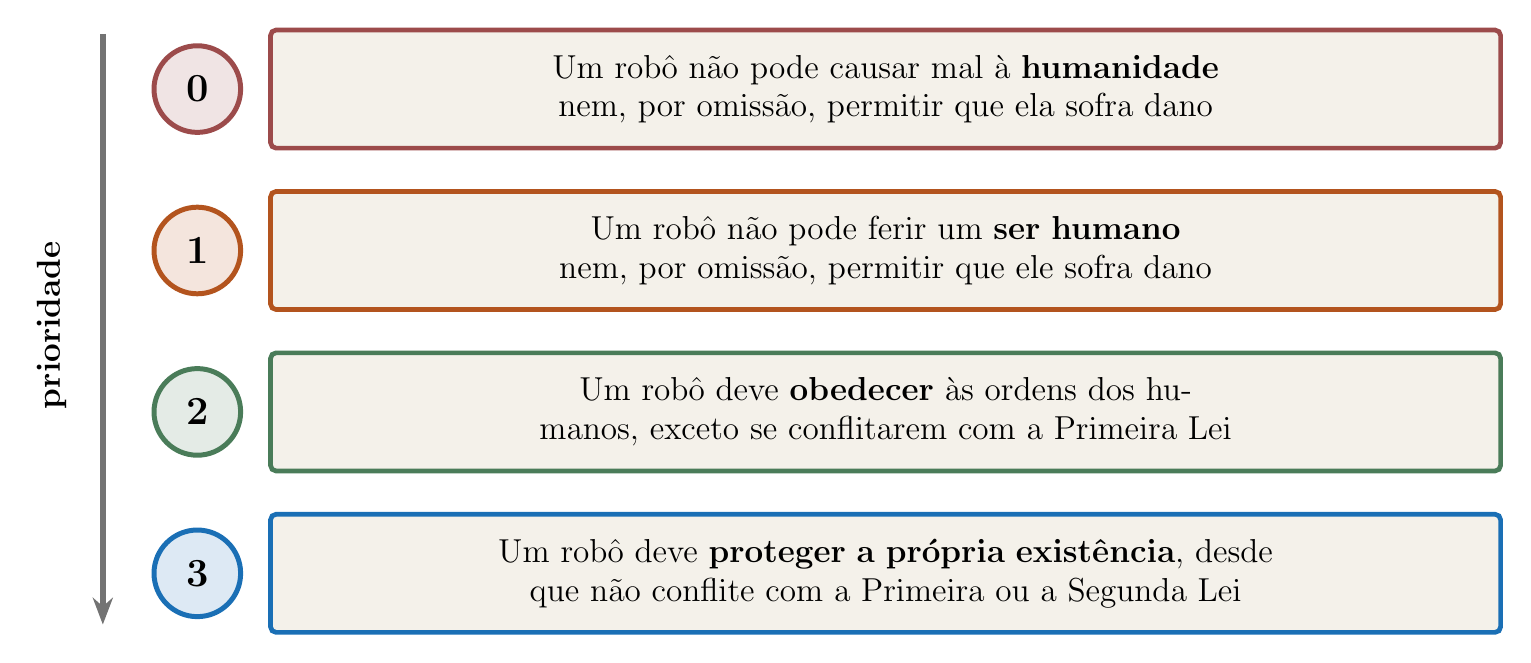
\begin{tikzpicture}[x=1cm,y=1cm]
\draw[black!55, line width=2.2pt, -{Stealth[length=3.4mm]}] (0.3,8.0) -- (0.3,0.5);
\node[font=\large\bfseries, rotate=90] at (-0.35,4.3) {prioridade};
\node[circle, draw=dred, fill=dred!15, line width=1.8pt, minimum size=1.1cm, font=\Large\bfseries] at (1.5,7.3) {0};
\node[dbox, draw=dred, line width=1.7pt, text width=15.2cm, minimum height=1.5cm, font=\large, anchor=west] at (2.4,7.3) {Um robô não pode causar mal à \textbf{humanidade} nem, por omissão, permitir que ela sofra dano};
\node[circle, draw=dorange, fill=dorange!15, line width=1.8pt, minimum size=1.1cm, font=\Large\bfseries] at (1.5,5.25) {1};
\node[dbox, draw=dorange, line width=1.7pt, text width=15.2cm, minimum height=1.5cm, font=\large, anchor=west] at (2.4,5.25) {Um robô não pode ferir um \textbf{ser humano} nem, por omissão, permitir que ele sofra dano};
\node[circle, draw=dgreen, fill=dgreen!15, line width=1.8pt, minimum size=1.1cm, font=\Large\bfseries] at (1.5,3.2) {2};
\node[dbox, draw=dgreen, line width=1.7pt, text width=15.2cm, minimum height=1.5cm, font=\large, anchor=west] at (2.4,3.2) {Um robô deve \textbf{obedecer} às ordens dos humanos, exceto se conflitarem com a Primeira Lei};
\node[circle, draw=dblue, fill=dblue!15, line width=1.8pt, minimum size=1.1cm, font=\Large\bfseries] at (1.5,1.1500000000000004) {3};
\node[dbox, draw=dblue, line width=1.7pt, text width=15.2cm, minimum height=1.5cm, font=\large, anchor=west] at (2.4,1.1500000000000004) {Um robô deve \textbf{proteger a própria existência}, desde que não conflite com a Primeira ou a Segunda Lei};
\end{tikzpicture}
\end{document}
